% !TEX root = ../Grunddatei.tex
\section{Methodology}

\subsection{Goals and tasks}
In this project, our main goal is to examine the potential and the limits of street analysis for freely available data sources. Those include open-source remote sensing data, specifically satellite images, as well as free ground-level imagery of streets and their surroundings. We aim to apply computer vision methods and technologies to detect street features, so that information about an area can be obtained and used for further analysis. The core of this project is to design and implement a workflow to connect satellite images, ground-level street view panoramas and deep learning systems in a combined automated application. For this, the project explores nuances of model capabilities in a combined setting, especially when given data (like satellite images or street view images) of varying quality.

As described, the main objective of this project is to create an application to automatically detect one-way streets in satellite imagery, based on ground-level views of found intersections. For that, we want to use different deep learning methods to approach the individual tasks. These include three major steps that can be used to group the different subtasks. The first task is the detection of an intersection in a given satellite image. The main purpose for this is to segment the area occupied by the intersection. This can be used in the second task, which includes the extraction of a street view panorama at the found intersection. Third, this 360-degree image is analysed for relevant sections of the panorama. Last, the detection of street signs relevant for one-way streets concludes the application.

\subsection{Used technologies}
A number of different tools, models and data sources are used to implement the individual tasks of the application. To get satellite images, the open-source remote sensing platform MapTiler is utilised. This service provides online maps, including satellite imagery of varying resolution, maps for data visualisation or schematic maps for specific use cases. For the proposed workflow, the \textit{MapTiler API} is used to get map tiles that can be combined into satellite images with a resolution of around 20cm per pixel \cite{Maptiler1}. The company offers a free access plan for non-commercial use that includes 100.000 API calls per month \cite{Maptiler2}. To get open-source street view panoramas, we are using \textit{Panoramax}, an open-source project dedicated to collecting and providing street level imagery. The free alternative to Google Street View was first founded by the French National Geographic Institute and includes over 74 million images, mostly focusing on French national territory. The project includes different instances that mostly provide different data. Each of those instances have individual API endpoints that are primarily used to search for, filter or download images and other data \cite{3panoramax}. In this project, the service is utilised to automatically locate and download 360-degree images at intersections that are detected in satellite images. Due to the data being geographically confined, the proposed workflow is developed and tested in a limited area. For this, we chose the French city of Caen, because of the density of available data in this region. Figure~\ref{fig:panoramax} shows the density of 360-degree panoramas available at Panoramax in Caen, Figure~\ref{fig:svp} illustrates an example for a specific street view panorama.

\begin{figure}[htbp]
    \centering
    
    \begin{minipage}{0.48\textwidth}
        \centering
        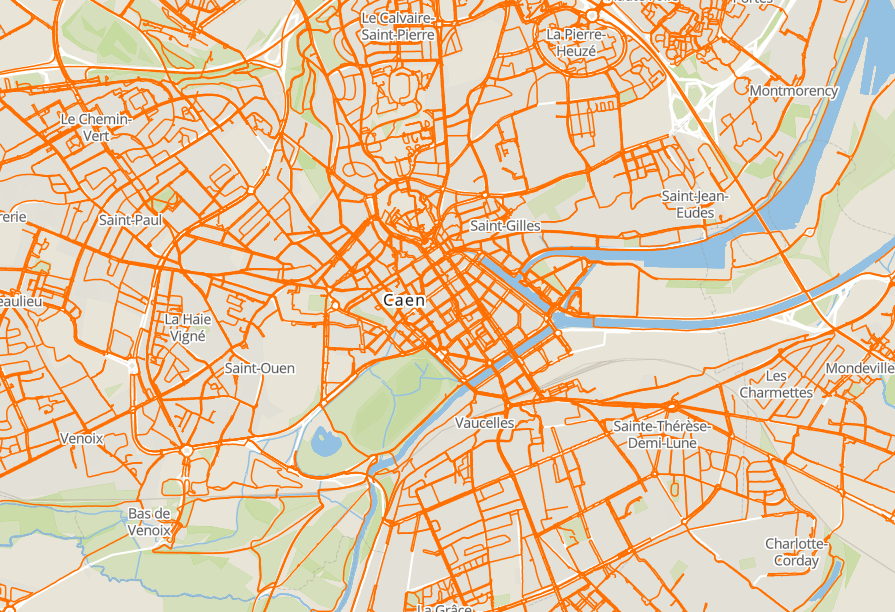
\includegraphics[width=\linewidth]{Pictures/panoramax_caen.png}
        \caption{Density of Panoramax street view images in Caen, France – source: api.panoramax.xyz}
        \label{fig:panoramax}
    \end{minipage}
    \hfill
    \begin{minipage}{0.48\textwidth}
        \centering
        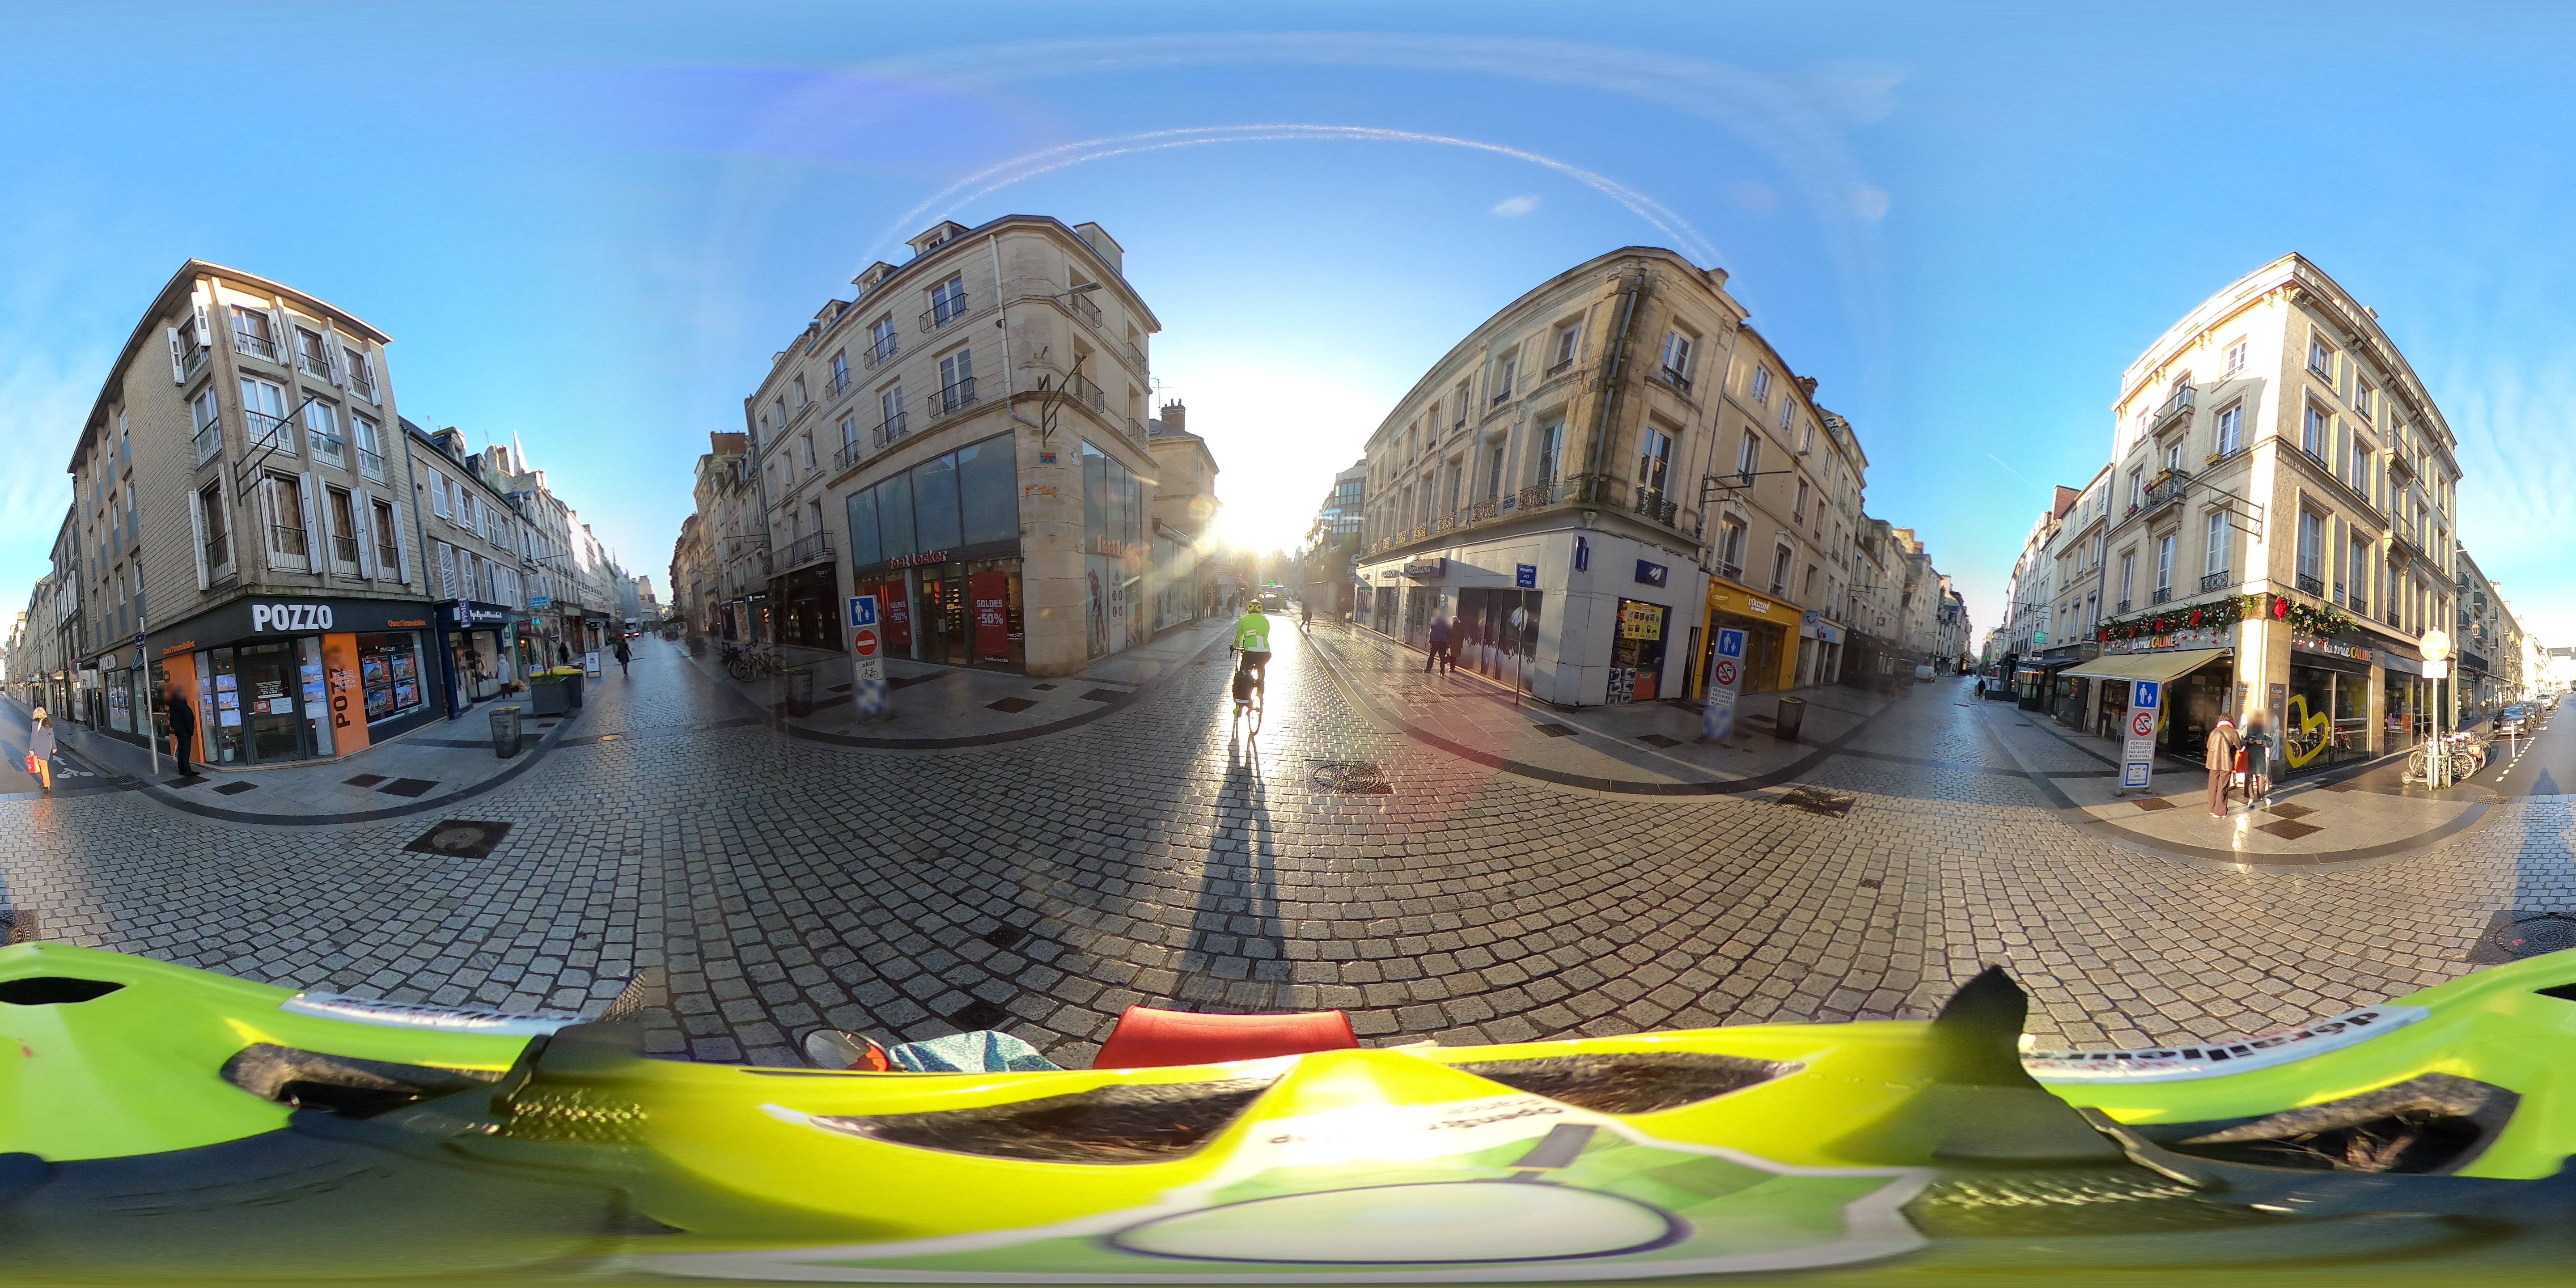
\includegraphics[width=\linewidth]{Pictures/svp_example.jpg}
        \caption{Example for street view panorama – source: api.panoramax.xyz, user: AlbaireN (uploaded 16.01.2025)}
        \label{fig:svp}
    \end{minipage}
    
\end{figure}

To analyse the collected images, the \textit{YOLO11} model by Ultralytics is used for the segmentation and detection task of the application. The model is characterised as an extension of classic convolutional neural networks that are often used for classic computer vision tasks, like object detection, classification or segmentation. The advancements of this technology are primarily because of changes in model architecture and lead to a very high computation and prediction speed while maintaining good accuracy \cite{4ultralytics}. Another factor for choosing YOLO11 for this project is the easy integration of the model into automated workflows as well as the results that get produced when running inference. Here, the produced data of segmentation and classification tasks include coordinates to identify relevant areas of a given image, which can be easily utilised for subsequent tasks. Another model called \textit{Depth Anything V2} is used for identifying relevant sections of the panorama image from Panoramax. This application is used to obtain a monocular depth estimation by producing a depth map of a given image \cite{5depthAnything}.

Other technologies are used in this project for creating custom datasets. The open-source platform \textit{Label Studio} is used to annotate data for machine learning processes \cite{6labelstudio}. To correctly segment intersections in the provided satellite images, we created a dataset containing 99 images with labelled intersection areas, which is used to fine-tune the applied YOLO11 model. To obtain the needed satellite images of intersections, we used a dataset from the French government office DINUM that included a detailed list of all intersections in France and their location, ordered by the respective départements (French administrative districts) \cite{7DINUM}. To combine all the tasks as a coherent implementation of the workflow, we use the programming language python.

\subsection{Proposed workflow}

The following flowchart (Figure~\ref{fig:flowchart}) presents all (sub-)tasks of the proposed application.

\begin{figure}[htbp]
    \centering
    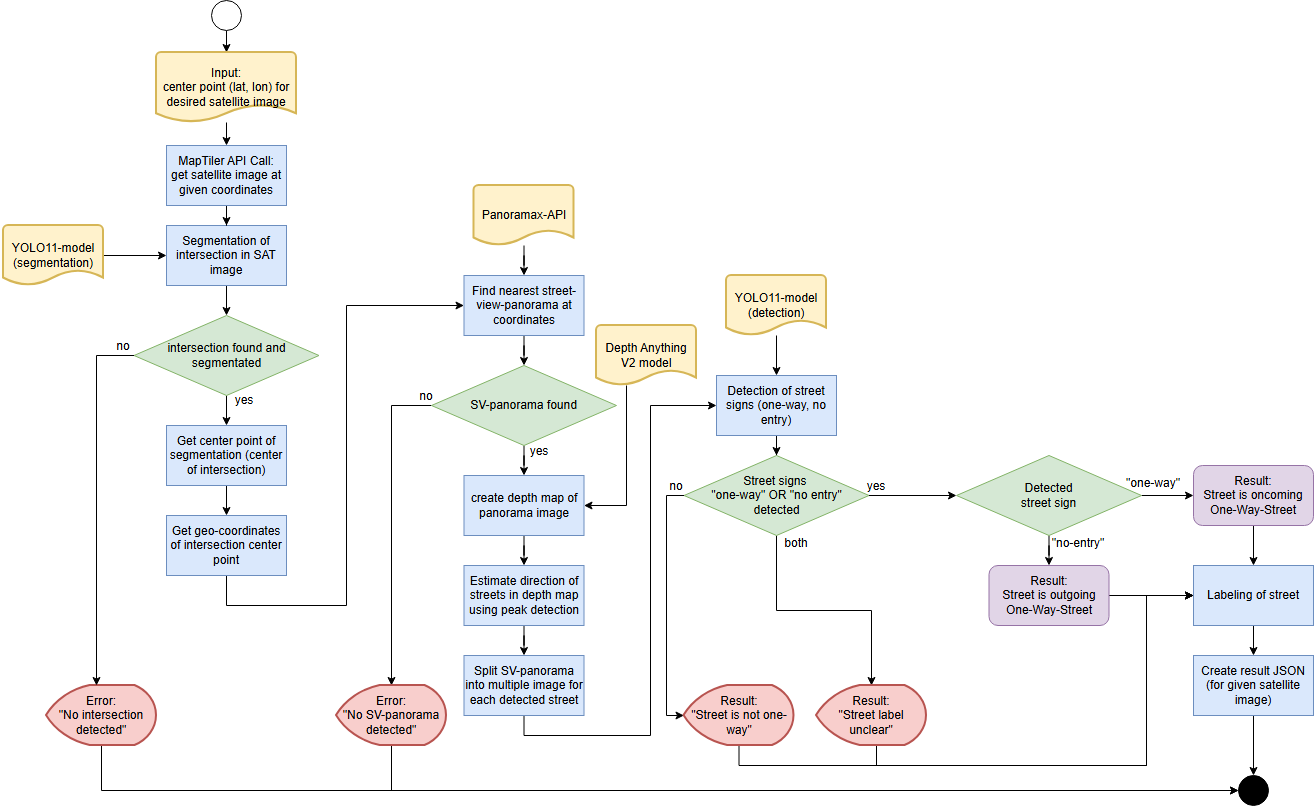
\includegraphics[width=\linewidth]{Pictures/flowchart.png}
    \caption{Flowchart of the proposed Workflow / Application – source: own depiction using draw.io}
    \label{fig:flowchart}
\end{figure}

The following section is dedicated to explaining specific subtasks of the application in further detail, starting with the identification of the intersection center point. For this, the output of the segmentation model (YOLO11) can be utilised. This YOLO11 model produces a polygon that represents the intersection area found in a given (satellite) image. This result is saved as a text file, which includes all coordinates of the segmentation polygon in the original image. Those coordinates represent specific normalised image pixels that define the edges of the polygon. Using this data, it is possible to obtain the mean value of the polygon, which represents the center point of the segmented area in the satellite image and thus, the center of the intersection. A comparison with the center point of the whole image allows the geographical coordinates of the intersection center point to be derived, since the image center always represents the provided coordinates from which the satellite image was formed. By calculating the distance, a single pixel corresponds to a real-world measurement and by determining the difference between both positions, it is possible to work out the coordinates of the segmentation center. A graphical depiction of the intersection center point detection is presented in Figure~\ref{fig:satImg_results}.

\begin{figure}[htbp]
    \centering
    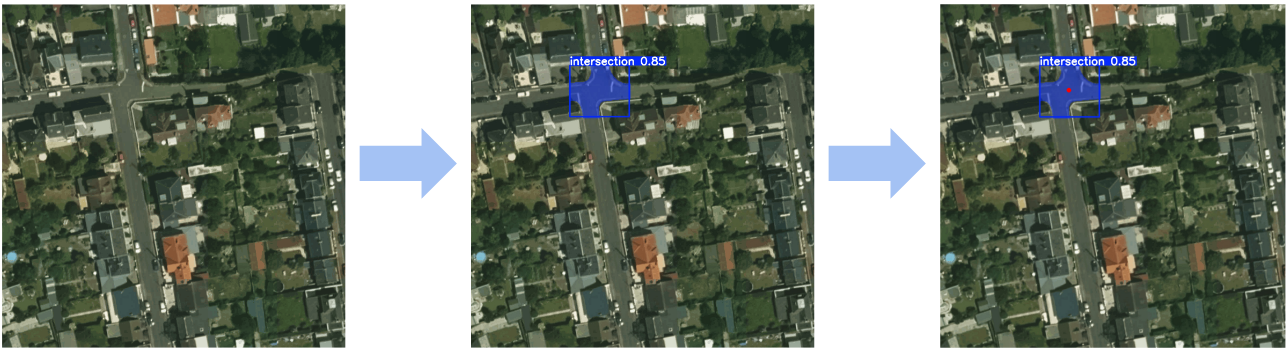
\includegraphics[width=\linewidth]{Pictures/satImg_results.png}
    \caption{Flowchart of the proposed Workflow / Application – source: own depiction using draw.io}
    \label{fig:satImg_results}
\end{figure}

SCHRITT FÜR DIE PEAK DETECTION

The other tasks can be implemented using simpler routines. For example, basic API requests with the python package \textit{requests} can be used to get data from individual MapTiler or Panoramax endpoints. This includes receiving satellite images and street view panoramas, as well as obtaining the nearest panorama image, given a specific location. The models included in the proposed workflow mostly require executing their respective prediction functions/commands with corresponding parameters. Last, saving the results of the analysis in JSON-files can also be done easily by utilising the python package \textit{json}.
